% Created by tikzDevice version 0.12.6 on 2026-09-22 03:17:05
% !TEX encoding = UTF-8 Unicode
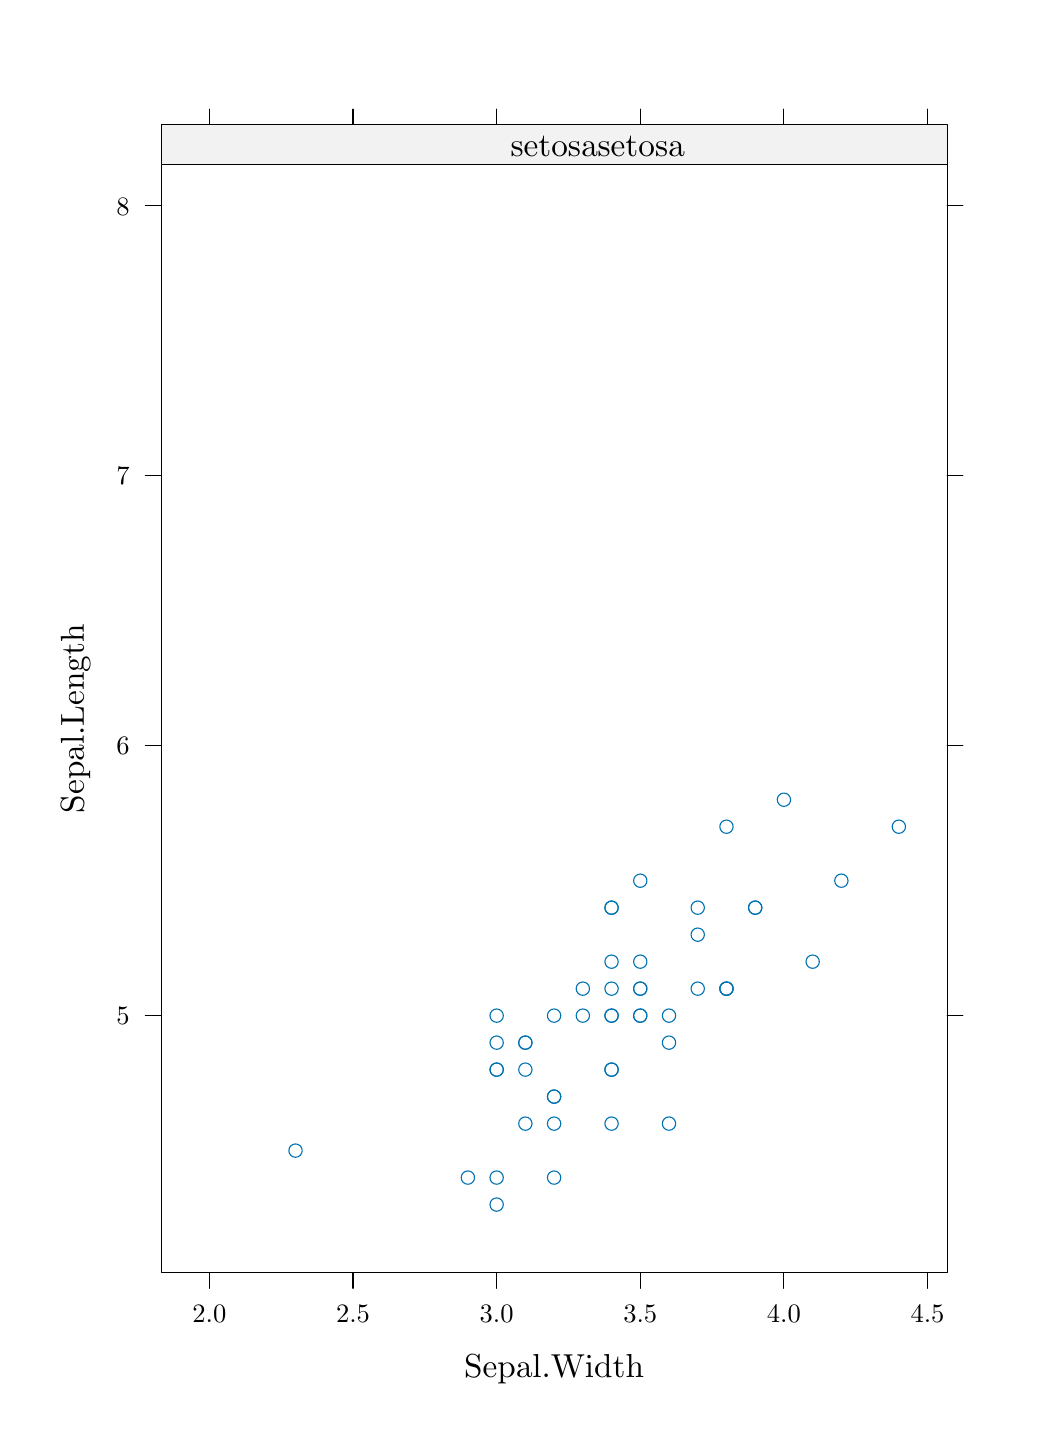
\begin{tikzpicture}[x=1pt,y=1pt]
\definecolor{fillColor}{RGB}{255,255,255}
\path[use as bounding box,fill=fillColor,fill opacity=0.00] (0,0) rectangle (361.35,505.89);
\begin{scope}
\path[clip] (  0.00,  0.00) rectangle (361.35,505.89);

\path[] (  0.00,  0.00) rectangle (361.35,505.89);
\definecolor{drawColor}{RGB}{0,0,0}

\node[text=drawColor,anchor=base,inner sep=0pt, outer sep=0pt, scale=  1.20] at (190.22, 18.07) {Sepal.Width};
\end{scope}
\begin{scope}
\path[clip] (  0.00,  0.00) rectangle (361.35,505.89);
\definecolor{drawColor}{RGB}{0,0,0}

\node[text=drawColor,rotate= 90.00,anchor=base,inner sep=0pt, outer sep=0pt, scale=  1.20] at ( 20.31,256.17) {Sepal.Length};
\end{scope}
\begin{scope}
\path[clip] (  0.00,  0.00) rectangle (361.35,505.89);
\definecolor{drawColor}{RGB}{0,0,0}

\path[draw=drawColor,line width= 0.4pt,line join=round,line cap=round] ( 65.64,470.75) -- ( 65.64,476.44);

\path[draw=drawColor,line width= 0.4pt,line join=round,line cap=round] (117.55,470.75) -- (117.55,476.44);

\path[draw=drawColor,line width= 0.4pt,line join=round,line cap=round] (169.46,470.75) -- (169.46,476.44);

\path[draw=drawColor,line width= 0.4pt,line join=round,line cap=round] (221.36,470.75) -- (221.36,476.44);

\path[draw=drawColor,line width= 0.4pt,line join=round,line cap=round] (273.27,470.75) -- (273.27,476.44);

\path[draw=drawColor,line width= 0.4pt,line join=round,line cap=round] (325.17,470.75) -- (325.17,476.44);
\end{scope}
\begin{scope}
\path[clip] (  0.00,  0.00) rectangle (361.35,505.89);
\definecolor{drawColor}{RGB}{0,0,0}

\path[draw=drawColor,line width= 0.4pt,line join=round,line cap=round] ( 48.20,148.89) -- ( 42.51,148.89);

\path[draw=drawColor,line width= 0.4pt,line join=round,line cap=round] ( 48.20,246.41) -- ( 42.51,246.41);

\path[draw=drawColor,line width= 0.4pt,line join=round,line cap=round] ( 48.20,343.94) -- ( 42.51,343.94);

\path[draw=drawColor,line width= 0.4pt,line join=round,line cap=round] ( 48.20,441.47) -- ( 42.51,441.47);

\node[text=drawColor,anchor=base east,inner sep=0pt, outer sep=0pt, scale=  0.96] at ( 36.82,145.58) {5};

\node[text=drawColor,anchor=base east,inner sep=0pt, outer sep=0pt, scale=  0.96] at ( 36.82,243.11) {6};

\node[text=drawColor,anchor=base east,inner sep=0pt, outer sep=0pt, scale=  0.96] at ( 36.82,340.64) {7};

\node[text=drawColor,anchor=base east,inner sep=0pt, outer sep=0pt, scale=  0.96] at ( 36.82,438.17) {8};
\end{scope}
\begin{scope}
\path[clip] (  0.00,  0.00) rectangle (361.35,505.89);
\definecolor{drawColor}{RGB}{0,0,0}

\path[draw=drawColor,line width= 0.4pt,line join=round,line cap=round] ( 65.64, 56.04) -- ( 65.64, 50.35);

\path[draw=drawColor,line width= 0.4pt,line join=round,line cap=round] (117.55, 56.04) -- (117.55, 50.35);

\path[draw=drawColor,line width= 0.4pt,line join=round,line cap=round] (169.46, 56.04) -- (169.46, 50.35);

\path[draw=drawColor,line width= 0.4pt,line join=round,line cap=round] (221.36, 56.04) -- (221.36, 50.35);

\path[draw=drawColor,line width= 0.4pt,line join=round,line cap=round] (273.27, 56.04) -- (273.27, 50.35);

\path[draw=drawColor,line width= 0.4pt,line join=round,line cap=round] (325.17, 56.04) -- (325.17, 50.35);

\node[text=drawColor,anchor=base,inner sep=0pt, outer sep=0pt, scale=  0.96] at ( 65.64, 38.05) {2.0};

\node[text=drawColor,anchor=base,inner sep=0pt, outer sep=0pt, scale=  0.96] at (117.55, 38.05) {2.5};

\node[text=drawColor,anchor=base,inner sep=0pt, outer sep=0pt, scale=  0.96] at (169.46, 38.05) {3.0};

\node[text=drawColor,anchor=base,inner sep=0pt, outer sep=0pt, scale=  0.96] at (221.36, 38.05) {3.5};

\node[text=drawColor,anchor=base,inner sep=0pt, outer sep=0pt, scale=  0.96] at (273.27, 38.05) {4.0};

\node[text=drawColor,anchor=base,inner sep=0pt, outer sep=0pt, scale=  0.96] at (325.17, 38.05) {4.5};

\path[draw=drawColor,line width= 0.4pt,line join=round,line cap=round] (332.23,148.89) -- (337.92,148.89);

\path[draw=drawColor,line width= 0.4pt,line join=round,line cap=round] (332.23,246.41) -- (337.92,246.41);

\path[draw=drawColor,line width= 0.4pt,line join=round,line cap=round] (332.23,343.94) -- (337.92,343.94);

\path[draw=drawColor,line width= 0.4pt,line join=round,line cap=round] (332.23,441.47) -- (337.92,441.47);
\end{scope}
\begin{scope}
\path[clip] ( 48.20, 56.04) rectangle (332.23,456.30);
\definecolor{drawColor}{RGB}{0,114,178}

\path[draw=drawColor,line width= 0.4pt,line join=round,line cap=round] (221.36,158.64) circle (  2.41);

\path[draw=drawColor,line width= 0.4pt,line join=round,line cap=round] (169.46,139.13) circle (  2.41);

\path[draw=drawColor,line width= 0.4pt,line join=round,line cap=round] (190.22,119.63) circle (  2.41);

\path[draw=drawColor,line width= 0.4pt,line join=round,line cap=round] (179.84,109.87) circle (  2.41);

\path[draw=drawColor,line width= 0.4pt,line join=round,line cap=round] (231.74,148.89) circle (  2.41);

\path[draw=drawColor,line width= 0.4pt,line join=round,line cap=round] (262.89,187.90) circle (  2.41);

\path[draw=drawColor,line width= 0.4pt,line join=round,line cap=round] (210.98,109.87) circle (  2.41);

\path[draw=drawColor,line width= 0.4pt,line join=round,line cap=round] (210.98,148.89) circle (  2.41);

\path[draw=drawColor,line width= 0.4pt,line join=round,line cap=round] (159.07, 90.37) circle (  2.41);

\path[draw=drawColor,line width= 0.4pt,line join=round,line cap=round] (179.84,139.13) circle (  2.41);

\path[draw=drawColor,line width= 0.4pt,line join=round,line cap=round] (242.12,187.90) circle (  2.41);

\path[draw=drawColor,line width= 0.4pt,line join=round,line cap=round] (210.98,129.38) circle (  2.41);

\path[draw=drawColor,line width= 0.4pt,line join=round,line cap=round] (169.46,129.38) circle (  2.41);

\path[draw=drawColor,line width= 0.4pt,line join=round,line cap=round] (169.46, 80.62) circle (  2.41);

\path[draw=drawColor,line width= 0.4pt,line join=round,line cap=round] (273.27,226.91) circle (  2.41);

\path[draw=drawColor,line width= 0.4pt,line join=round,line cap=round] (314.79,217.16) circle (  2.41);

\path[draw=drawColor,line width= 0.4pt,line join=round,line cap=round] (262.89,187.90) circle (  2.41);

\path[draw=drawColor,line width= 0.4pt,line join=round,line cap=round] (221.36,158.64) circle (  2.41);

\path[draw=drawColor,line width= 0.4pt,line join=round,line cap=round] (252.51,217.16) circle (  2.41);

\path[draw=drawColor,line width= 0.4pt,line join=round,line cap=round] (252.51,158.64) circle (  2.41);

\path[draw=drawColor,line width= 0.4pt,line join=round,line cap=round] (210.98,187.90) circle (  2.41);

\path[draw=drawColor,line width= 0.4pt,line join=round,line cap=round] (242.12,158.64) circle (  2.41);

\path[draw=drawColor,line width= 0.4pt,line join=round,line cap=round] (231.74,109.87) circle (  2.41);

\path[draw=drawColor,line width= 0.4pt,line join=round,line cap=round] (200.60,158.64) circle (  2.41);

\path[draw=drawColor,line width= 0.4pt,line join=round,line cap=round] (210.98,129.38) circle (  2.41);

\path[draw=drawColor,line width= 0.4pt,line join=round,line cap=round] (169.46,148.89) circle (  2.41);

\path[draw=drawColor,line width= 0.4pt,line join=round,line cap=round] (210.98,148.89) circle (  2.41);

\path[draw=drawColor,line width= 0.4pt,line join=round,line cap=round] (221.36,168.39) circle (  2.41);

\path[draw=drawColor,line width= 0.4pt,line join=round,line cap=round] (210.98,168.39) circle (  2.41);

\path[draw=drawColor,line width= 0.4pt,line join=round,line cap=round] (190.22,119.63) circle (  2.41);

\path[draw=drawColor,line width= 0.4pt,line join=round,line cap=round] (179.84,129.38) circle (  2.41);

\path[draw=drawColor,line width= 0.4pt,line join=round,line cap=round] (210.98,187.90) circle (  2.41);

\path[draw=drawColor,line width= 0.4pt,line join=round,line cap=round] (283.65,168.39) circle (  2.41);

\path[draw=drawColor,line width= 0.4pt,line join=round,line cap=round] (294.03,197.65) circle (  2.41);

\path[draw=drawColor,line width= 0.4pt,line join=round,line cap=round] (179.84,139.13) circle (  2.41);

\path[draw=drawColor,line width= 0.4pt,line join=round,line cap=round] (190.22,148.89) circle (  2.41);

\path[draw=drawColor,line width= 0.4pt,line join=round,line cap=round] (221.36,197.65) circle (  2.41);

\path[draw=drawColor,line width= 0.4pt,line join=round,line cap=round] (231.74,139.13) circle (  2.41);

\path[draw=drawColor,line width= 0.4pt,line join=round,line cap=round] (169.46, 90.37) circle (  2.41);

\path[draw=drawColor,line width= 0.4pt,line join=round,line cap=round] (210.98,158.64) circle (  2.41);

\path[draw=drawColor,line width= 0.4pt,line join=round,line cap=round] (221.36,148.89) circle (  2.41);

\path[draw=drawColor,line width= 0.4pt,line join=round,line cap=round] ( 96.79,100.12) circle (  2.41);

\path[draw=drawColor,line width= 0.4pt,line join=round,line cap=round] (190.22, 90.37) circle (  2.41);

\path[draw=drawColor,line width= 0.4pt,line join=round,line cap=round] (221.36,148.89) circle (  2.41);

\path[draw=drawColor,line width= 0.4pt,line join=round,line cap=round] (252.51,158.64) circle (  2.41);

\path[draw=drawColor,line width= 0.4pt,line join=round,line cap=round] (169.46,129.38) circle (  2.41);

\path[draw=drawColor,line width= 0.4pt,line join=round,line cap=round] (252.51,158.64) circle (  2.41);

\path[draw=drawColor,line width= 0.4pt,line join=round,line cap=round] (190.22,109.87) circle (  2.41);

\path[draw=drawColor,line width= 0.4pt,line join=round,line cap=round] (242.12,178.14) circle (  2.41);

\path[draw=drawColor,line width= 0.4pt,line join=round,line cap=round] (200.60,148.89) circle (  2.41);
\end{scope}
\begin{scope}
\path[clip] (  0.00,  0.00) rectangle (361.35,505.89);
\definecolor{drawColor}{RGB}{0,0,0}

\path[draw=drawColor,line width= 0.4pt,line join=round,line cap=round] ( 48.20, 56.04) rectangle (332.23,456.30);
\end{scope}
\begin{scope}
\path[clip] ( 48.20,456.30) rectangle (332.23,470.75);
\definecolor{drawColor}{gray}{0.95}
\definecolor{fillColor}{gray}{0.95}

\path[draw=drawColor,line width= 0.4pt,line join=round,line cap=round,fill=fillColor] ( 48.20,456.30) rectangle (332.23,470.75);
\definecolor{drawColor}{RGB}{0,0,0}

\node[text=drawColor,anchor=base west,inner sep=0pt, outer sep=0pt, scale=  1.20] at (174.49,459.39) {\hypertarget{setosa}{setosa}};
\end{scope}
\begin{scope}
\path[clip] (  0.00,  0.00) rectangle (361.35,505.89);
\definecolor{drawColor}{RGB}{0,0,0}

\path[draw=drawColor,line width= 0.4pt,line join=round,line cap=round] ( 48.20,456.30) rectangle (332.23,470.75);
\end{scope}
\end{tikzpicture}
